% sample.tex
\documentclass[graduation-thesis]{jsarticle}
	\usepackage[dvipdfmx]{graphicx}
	\usepackage{url}
	\usepackage{atbegshi}
	\AtBeginShipoutFirst{\special{pdf:tounicode EUC-UCS2}}
	\usepackage[dvipdfmx,setpagesize=false]{hyperref}
		\usepackage[dvipdfmx]{color}
\usepackage{url}
\usepackage{float}
\usepackage[setpagesize=false]{hyperref}
\usepackage{ascmac}
\usepackage{here}
\usepackage{txfonts}
\usepackage{listings, jlisting}
\author{61305507 情報工学科 勝又裕之}
\date{\today}
\title{}
\begin{document}


\makeatletter
\renewcommand{\thetable}{
	\thesection.\arabic{table}
} %「表(章番号)-#.」と表記するための措置
\@addtoreset{table}{section}

\renewcommand{\thefigure}{
	\thesection.\arabic{figure}
}
\@addtoreset{figure}{section} %「図(章番号)-#.」と表記するための措置

\setcounter{page}{1}

\pagenumbering{roman}
\tableofcontents
\clearpage

\pagenumbering{arabic}

\definecolor{keywords}{RGB}{255,0,90}
\definecolor{comments}{RGB}{0,0,113}
\definecolor{red}{RGB}{160,0,0}
\definecolor{green}{RGB}{0,150,0}
\lstset{
	basicstyle=\ttfamily\footnotesize,
	frame=single,
	keywordstyle=\color{keywords},
	commentstyle=\color{comments},
	stringstyle=\color{red},
	showstringspaces=false,
	identifierstyle=\color{green},
	}

\section{はじめに}
\label{intro}
 近年,マルチテナント型のクラウドにコンテナ技術が利用されている.マルチテナント型のクラウドの例として, Amazon Web Services や Google Cloud Platform がある.こういったクラウドを管理する場合に, isolation が重要である.ここで,isolation と throttle との違いを明確にしておく.ディスクへの書き込みを 15\% に制限しているが, 30\% 必要としているプロセスと, 85\% に制限しているが 50\% しか必要としていないプロセスを実行したとする.throttle であれば,前者はディスクへの書き込みを 15\% ,後者は 50\% の割合で使う.一方, isolation では,余っている分を自由に利用できるので,後者が 50\% しか利用していないため,前者は必要としている 30\% 分を使うことができる.\\
\begin{figure}[H]
	\begin{center}
		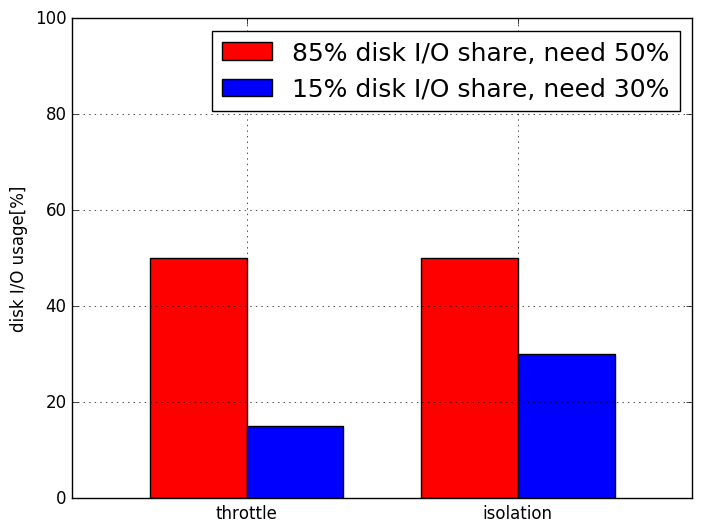
\includegraphics[width=7.5cm]{images/isolation.png}
		\caption{throttle と isolation との違い}
		\label{fig:isolation}
	\end{center}
\end{figure}
 コンテナ技術の一つとして, Linux コンテナ (LXC) がある.LXC は linux カーネル機能の一つである cgroup を利用して,コンテナ毎の資源管理を行っている.また,それによってコンテナ間の isolation を保っている.しかし, cgroup による isolation は不完全である.2個のコンテナを用意する.片方のコンテナでは cgroup によって disk I/O 使用率を 85\% に制限し,Flexible IO(FIO) write benchmark を実行する.もう一方のコンテナでは,disk I/O 使用率を 15\% に制限し,FIO write benchmark を 100 命令に一回 fsync しながら実行する.この状況では,disk I/O 使用率を 85\% に制限している方は,本来は 85\% 使えるはずが 40\% しか使えなかった.\\
 コンテナ環境における isolation の不完全性は, DDoS 攻撃への脆弱性となる可能性がある.本論文では,実際にコンテナ環境において利用される, MySQL と varmail に対して攻撃が可能であることを示し,その解析を行う.MySQL への攻撃が可能であるか検証するためコンテナを2つ用意する.片方のコンテナで, disk I/O 使用率を 85\% に制限して MySQL benchmark を実行する.もう一方のコンテナで, disk I/O 使用率を 15\% に制限して,ファイルのメタデータを頻繁に更新するスクリプトと FIO read benchmark を実行する. この時, MySQL は,本来 disk I/O を 85\% 使えるはずが,50\% しか使えていなかった.よって, MySQL に対して攻撃が可能だと言える.同様に, varmail への攻撃が可能であるか検証するためにコンテナを2つ用意する.片方のコンテナで disk I/O 使用率を 85\% に制限して varmail benchmark を実行する.もう一方のコンテナで, disk I/O 使用率を 15\% に制限して,ファイルのメタデータを頻繁に更新するスクリプトと FIO read benchmark を実行する.この時, varmail は,本来 disk I/O を 85\% 使えるはずが, 50\% しか使えていなかった.よって, varmail に対して攻撃が可能だと言える.\\
 cgroup による isolation が不完全な原因は,journal であった.LXC ではコンテナ間で file system を共有しているため,複数のコンテナの disk I/O が,一つの journal でシリアライズされる.攻撃側は,頻繁に fsync を呼び,メタデータを更新しようとしている.攻撃側の頻繁な更新リクエストにより, journal に負荷がかかる.これによって, disk I/O の遅延時間が増加するようになるが,一つの journal で管理していることによって,すべてのコンテナでこの影響を受ける.したがって,攻撃対象の遅延時間を増やし,パフォーマンスを下げることが出来たのだと考える.また,攻撃側の,メタデータの更新リクエストの頻度を上げるほど,攻撃対象の遅延時間は増加する傾向にあった.\\
 本論文の構成を以下に示す.
 第\ref{sec:LXC}章では,LXC の資源管理の仕組みについて説明する.
 第\ref{sec:journaling}章では,journaling file system の仕組みについて説明する.
 第\ref{sec:DDoS}章では,現在のコンテナ環境において, DDoS 攻撃が可能であることを示す.
 第\ref{analysis}章では, DDoS 攻撃が可能である原因を解析する.
 第\ref{relative}章では,本研究に関連する研究について紹介する.
 第\ref{conclusion}章では,まとめと今後の課題について述べる.
 
\clearpage
\section{Linux コンテナにおける資源管理}
\label{sec:LXC}
 近年,仮想化技術としてコンテナが注目されている.コンテナを実現する技術の一つに Linux コンテナ (LXC) がある.本章では, LXC の資源管理の仕組みについて説明をする.\\
 LXC は,一つのマシン上にコンテナという隔離空間を作り出す.LXC は, Linux カーネル機能の一つである cgroup を使い,コンテナへの資源の割り当てを管理している.\\
 cgroup は, OS が管理する資源を一元的に管理できる Linux カーネル機能である.cgroup は,プロセス,ファイルシステム, CPU ,メモリ, block I/O デバイスなどの各種デバイスといった多種のものを管理できる. cgroup はサブシステムによって,これら資源を管理している.表\ref{tb:subsystem}に, cgroup のサブシステムとその機能を示す.\\
\begin{table}[htb]
	\begin{center}
		\caption{cgroup のサブシステムとその機能}
		\begin{tabular}{|c||l|} \hline
			サブシステム名 & 機能\\
			\hline \hline
			blkio & ブロックデバイスへの入出力アクセスの制限を設定する\\
			\hline
			cpu & CPU コアの時間配分の割合を設定する\\
			\hline
			cpuacct & タスクが消費する CPU 時間をレポートする\\
			\hline
			cpuset & 使用可能な CPU コア数を設定する\\
			\hline
			devices & デバイスへのアクセスを制御する\\
			\hline
			freezer & タスクの一時停止と再開を制御する\\
			\hline
			hugetlb & cgroup からの hugetlb の使用\\
			\hline
			memory & タスクによって使用されるメモリの制限を設定する\\
			\hline
			net\_cls & プロセスが発信するパケットに識別子を付与し,制御する\\
			\hline
			net\_prio & タスクのネットワークの優先度を動的に設定する\\
			\hline
			pids & 起動するプロセス数を制限する\\
			\hline
		\end{tabular}
		\label{tb:subsystem}
	\end{center}
\end{table}
 cgroup は資源のグループ化を行い,グループごとに資源利用の優先度を決めたり,利用できる資源を制限したりしている.さらに,グループを隔離することで,他のグループから中が見えないようにしている.これによって,コンテナという隔離空間を作り出している.したがって,図\ref{fig:grouping}のように,あるコンテナから他のコンテナの内部へはアクセスが出来ない.
\begin{figure}[H]
	\begin{center}
		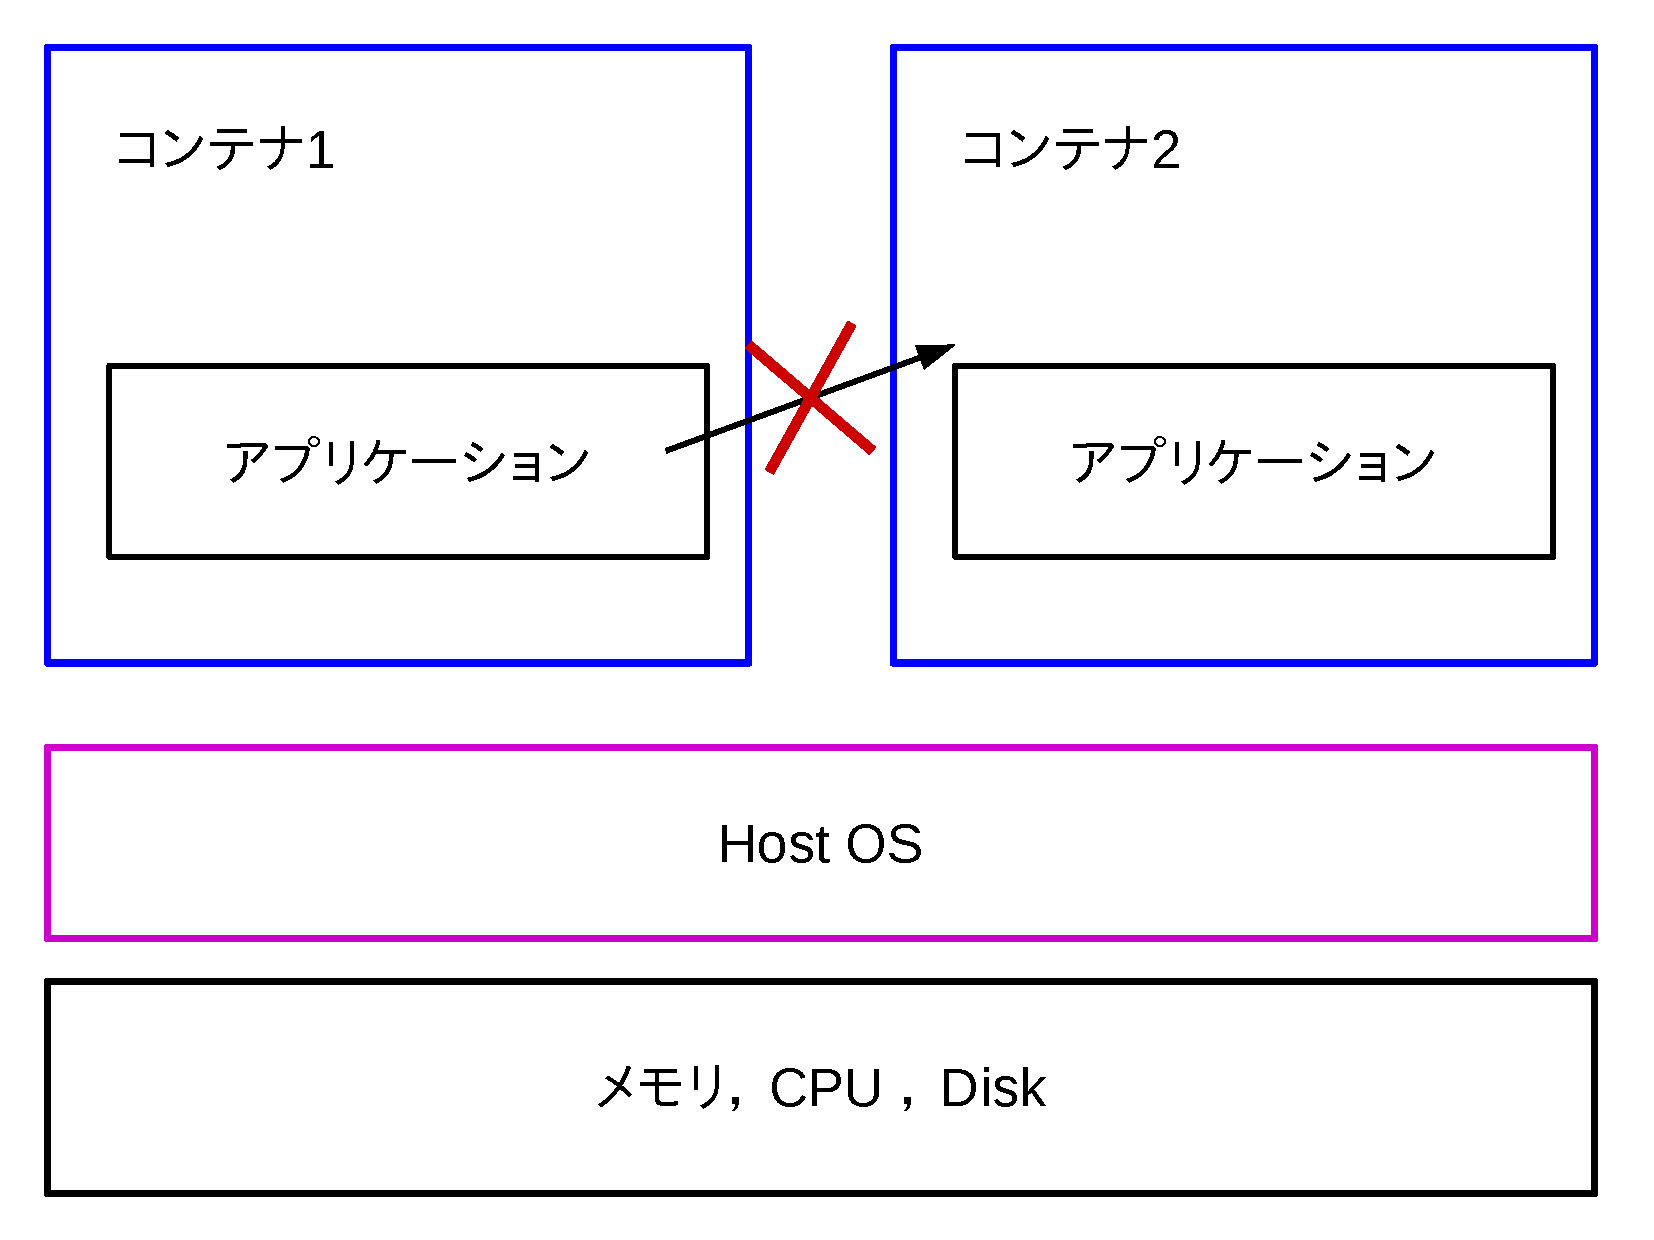
\includegraphics[width=5.0cm, clip]{images/kakuri.pdf}
		\caption{cgroup によるグループ化}
		\label{fig:grouping}
	\end{center}
\end{figure}
 より詳しく見ていくために, blkio サブシステムについて説明する。blkio サブシステムは, cgroup 内のタスクが行う,ブロックデバイス上の I/O アクセスを管理します.制御の方法は,重み付け比例配分という方法と, I/O スロットリングという方法の2種類があります.I/O スロットリングは,特定のデバイスへの I/O 操作数の上限を設定するのに使います.重み付け比例配分は, Completely Fair Queuing スケジューラによりスケジューリングを行うことで,グループに重み付けをすることができる.この重み付けは, 100 ~ 1000 の間で指定できる.\\
 例えば,2つのグループがあり,これらをグループ A とグループ B とする.グループ A とグループ B のブロックデバイスへの I/O アクセスを 2 : 1 に重み付けしたい場合, グループ A に対応する blkio サブシステム以下の blkio.weight の値を 1000 に設定し,グループ B に対応する blkio サブシステム以下の blkio.weight の値を 500 に設定する.これによって, 1000 : 500 、つまり 2 : 1 で重み付けをすることができる.
 
\clearpage
\section{journaling file system}
\label{sec:journaling}
 唐突な電源断が発生したり, OS にバグが発生したりすると, file system の一貫性が失われてしまう.この問題を crash-consistency problem という.本来,保存してあるデータは永続的なものであるべきである.そこで,この問題を解決するために生み出されたものが, journaling file system である.本章では, ext4 file system において,デフォルトで用いられている, metadata journaling について説明する.
\subsection{journaling の意味}
 本来,データは永続的なものであるべきである。しかし,データを変更する途中で,電源断が発生したり OS にバグが発生したりして,変更が中断されてしまう場合が存在する.この場合,復帰する際に特別な操作を行わないと, file system に矛盾が生じてしまう.簡単な書き込みを例に,途中でクラッシュが起こってしまった場合にどうなるかを紹介する.書き込み例は,すでに存在するファイルに対して,データブロックを一つ加えるもので,ファイルを開く,正しいオフセットの位置まで移動する, 4KB の write を発行する,ファイルを閉じるの 4 つの操作からなる.\\
 書き込み対象の file system も標準的な, inode bitmap, data bitmap, inodes, data blocks を含んでいるものとする.データ構造の初期状態を図\ref{fig:data1}に示す.inode bitmap Ba は,inode I[v1] が使用中であることを示している.data bitmap B[v1] は,data block Da が使用中であることを示している.inode I[v1] は,file size が 1 であり,ファイルの内容がブロック 4 ,つまり data block Da に格納されていることを示している.data block Da は,ファイルの内容を格納している.\\
\begin{figure}[H]
	\begin{center}
		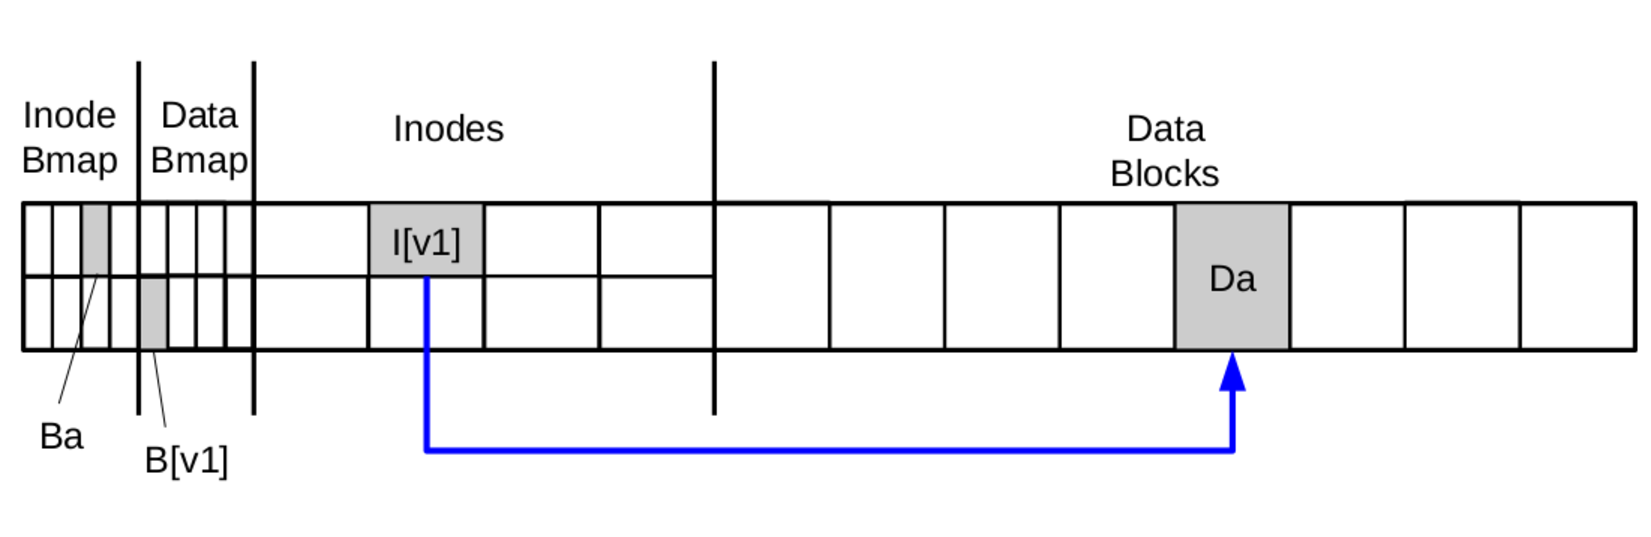
\includegraphics[width=15.0cm,clip]{images/data1.pdf}
		\caption{初期のデータ構造}
		\label{fig:data1}
	\end{center}
\end{figure}
 また, inode I[v1]の中身は表\ref{tab:inode1}のようになっているとする.\\
% この直後の表が来ないため,形を整える必要があるかもしれない.
\begin{table}[h]
	\begin{center}
	\caption{inode の初期状態}
		\begin{tabular}{lcl}
			owner & : & hoge \\
			permissions & : & read-write \\
			size & : & 1 \\
			pointer & : & 4 \\
			pointer & : & null \\
			pointer & : & null \\
			pointer & : & null
		\end{tabular}
		\label{tab:inode1}
	\end{center}
\end{table}
 1 ブロック分が割り当てられているので file size は 1, pointer はブロック 4 を指している.ここに,簡単な書き込み操作を行うと, data bitmap, inode, data block の 3 箇所が更新される.data block では,新しく data block Db が,ファイルに割り当てられる.inode I[v1] の pointer が,元々割り当てられている data block Da 以外に,新しく割り当てられた data block Db も指すようになり,file size は 2 となる.さらに, 新しく data bitmap B[v2] が, data block Db が使用されていることを指し示すようにする.無事,書き込み操作が行われた場合, inode I[v1] は表\ref{tab:inode2}のようなる.\\
\begin{table}[h]
	\begin{center}
	\caption{inode の書き込み操作終了後の状態}
		\begin{tabular}{lcl}
			owner & : & hoge \\
			permissions & : & read-write \\
			size & : & 2 \\
			pointer & : & 4 \\
			pointer & : & 5 \\
			pointer & : & null \\
			pointer & : & null
		\end{tabular}
		\label{tab:inode2}
	\end{center}
\end{table}
 さらに,書き込み操作終了後のデータ構造は図\ref{fig:data2}のようになる.\\
\begin{figure}[H]
	\begin{center}
		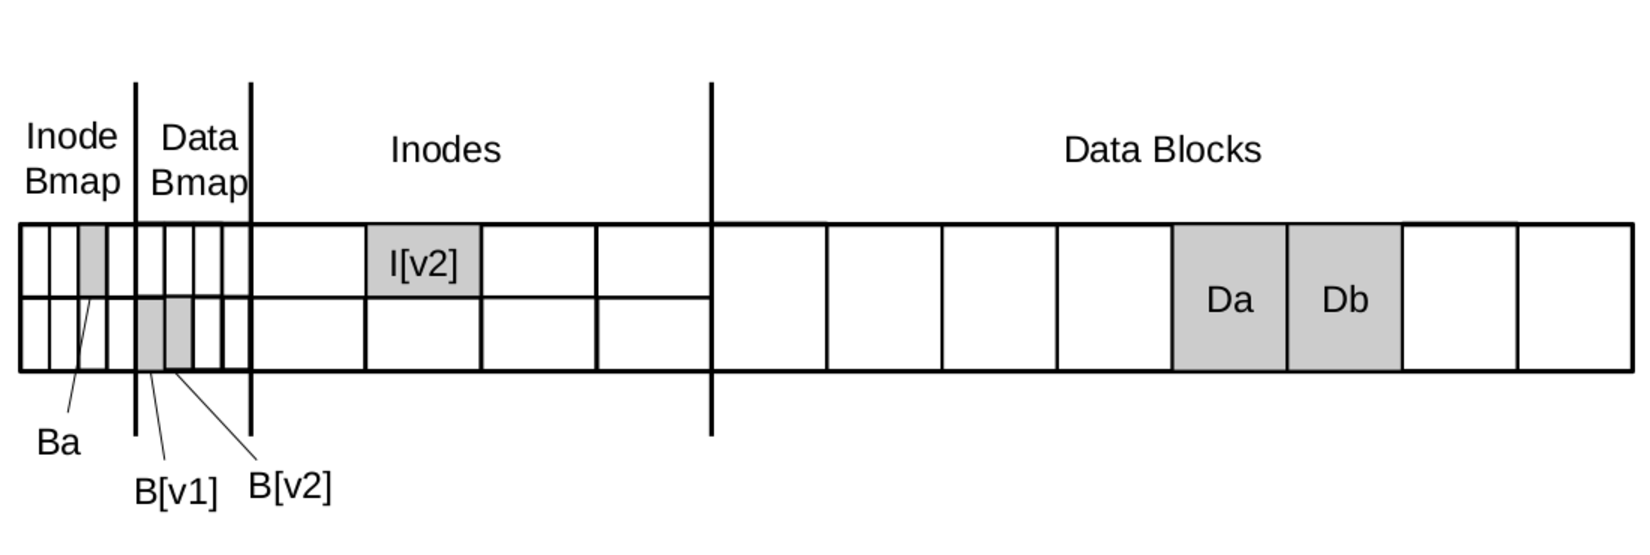
\includegraphics[width=15.0cm,clip]{images/data2.pdf}
		\caption{書き込み終了後のデータ構造}
		\label{fig:data2}
	\end{center}
\end{figure}
 上記で述べたとおり,書き込みの際に更新するのは,data bitmap, inode, data block の 3 箇所である.3 箇所の内, 1 箇所のみ,または 2 箇所の更新が終わった時点で,障害が発生した場合を説明する.
\begin{description}
	\item[data block Db のみ書き込みが完了した場合]\mbox{}\\
 この場合,データは disk に書き込まれているが, inode はそのブロックを指し示していない.さらに, data bitmap を見ても,そのブロックが使用されていないと表示されている.これは,書き込み操作が行われなかった場合とほぼ同じであるため,問題がないと言える.
	\item[inode I[v2] のみ書き込みが完了した場合]\\
	\item[data bitmap B[v2] のみ書き込みが完了した場合]\\
	\item[inode I[v2] と data bitmap B[v2] のみ書き込みが完了した場合]\\
	\item[inode I[v2] と data block Db のみ書き込みが完了した場合]\\
	\item[data bitmap B[v2] と data block Db のみ書き込みが完了した場合]\\
\end{description}
\subsection{journaling の手順}

\clearpage
\section{Linux コンテナに対する DDoS 攻撃}
\label{sec:DDoS}

\clearpage
\section{コンテナにおける資源管理の脆弱性解析}
\label{sec:analysis}

\clearpage
\section{関連研究}
\label{sec:relative}

\clearpage
\section{まとめ}
\label{sec:conclusion}

\end{document}